\documentclass[12pt,letterpaper]{article}

\usepackage{amsmath, amsthm}
\usepackage{graphicx,hyperref}
\usepackage{microtype, parskip}
\usepackage[numbers,sort&compress]{natbib}
\usepackage{lineno}
\usepackage[font=small]{caption}
\usepackage{subcaption, multirow, morefloats}
\usepackage{subcaption, wrapfig}
\usepackage{titlesec}
\usepackage[nottoc,numbib]{tocbibind}
\usepackage{authblk, attrib, fullpage}
\usepackage{lineno}

\frenchspacing

\captionsetup[subfigure]{position = top, labelfont = bf, textfont = normalfont, singlelinecheck = off, justification = raggedright}

\renewcommand{\section}[1]{%
\bigskip
\begin{center}
\begin{Large}
\normalfont\scshape #1
\medskip
\end{Large}
\end{center}}

\renewcommand{\subsection}[1]{%
\bigskip
\begin{center}
\begin{large}
\normalfont\itshape #1
\end{large}
\end{center}}

\renewcommand{\subsubsection}[1]{%
\vspace{2ex}
\noindent
\textit{#1.}---}

\renewcommand{\tableofcontents}{}

\bibpunct{(}{)}{;}{a}{}{,}  % this is a citation format command for natbib

\title{How cryptic is cryptic diversity? Machine learning approaches to classifying morphological variation in \textit{Emys marmorata} (Testudinoidea, Emydidae).}
\author[1]{Peter D Smits}%\thanks{psmits@uchicago.edu}}
\author[1,2]{Kenneth D Angielczyk}%\thanks{kangielczyk@fieldmuseum.org}}
\author[3]{James F Parham}%\thanks{jparham@fullerton.edu}}
\affil[1]{Committee on Evolutionary Biology, University of Chicago}
\affil[2]{Integrative Research Center, Field Museum of Natural History}
\affil[3]{Department of Geological Sciences, California State University -- Fullerton}


\begin{document}
\maketitle
\noindent{\textbf{Corresponding author:} Peter D Smits, Committee on Evolutionary Biology, University of Chicago, 1025 E. 57th Street, Culver Hall 402, Chicago, IL, 60637, USA; E-mail: \href{mailto:psmits@uchicago.edu}{psmits@uchicago.edu}}

\linenumbers
\modulolinenumbers[2]

\begin{abstract}
\end{abstract}

\section{Introduction}

\section{Materials and Methods}
\subsection{Specimens and sampling}
We collected landmark-based morphometric data from SAMPLE adult \textit{E. marmorata} museum specimens. These specimens include both newly sampled individuals and those sampled in previous studies of plastral shape variation \citep{Angielczyk2007,Angielczyk2011,Angielczyk2013a}. 

Specimen classification was based on known specimen geographic information which was recorded from museum collection information. When precise latitude and longitude information was not available it was estimated from whatever locality information was present. Because the specimens used to define the subclades in \citet{Spinks2005} and \citet{Spinks2010} were not available for study, all specimen classifications were based solely on this geographic information and not from explicit assignment in previous studies. Instead, classification was based on matching museum locality data with the geographic boundaries of the molecularly-defined clades of \citet{Spinks2005} and \citet{Spinks2010}. Because the exact barriers between different biogeographic regions are unknown and unclear, two assignments for both the morphologically and molecularly based hypotheses were used. Each morphologically based hypothesis had three classes, while each molecular-based had four classes. In total, each specimen was given four different classifications. 


\subsection{Geometric morphometrics}
Following previous work on plastral variation \citep{Angielczyk2007,Angielczyk2011,Angielczyk2013a}, 19 landmarks were digitized using TpsDig 2.04 \citep{Rohlf2005}. These landmarks were chosen to maximize the description of general plastral variation(Fig. \ref{fig:plastra}). 17 of these landmarks are at the endpoints or intersection of the keratinous plastral scutes that cover the platron. 12 of these landmarks were chosen to be symmetrical across the axis of symmetry and, in order to prevent degrees of freedom and other concerns \citep{Klingenberg2002}, prior to analysis these landmarks were reflected across the axis of symmetry (i.e. midline) and the average position of each symmetrical pair was used. In cases where damage or incompleteness prevented symmetric landmarks from being determined, only the single member of the pair was used. Analysis was conducted on the resulting ``half'' plastra. Plastral landmark configurations were superimposed using generalized Procrustes analysis \citep{Dryden1998a} after which, the principal components (PC) of shape were calculated. This was done using the \texttt{shapes} package for R \citep{2013,Dryden2013}.


\subsection{Machine learning analyses}
\subsubsection{Unsupervised learning}
In order to preserve the relationship between all landmark configurations in shape space, the dissimilarity between observations was measured using Kendall's Riemanninan shape distance or \(\rho\) \citep{Kendall1984a,Dryden1998a}. This metric was chosen because shape space, or the set of all possible shape configurations following Procrustes superimposition, is a Riemannian manifold and thus non-Euclidean \citep{Dryden1998a}. \(\rho\) varies between 0 and \(\pi / 2\) when there is no reflection invariance, which should not be a concern in the case of the half plastral landmark configurations used in the study.

The \(\rho\) dissimilarity matrix was divisively clustered using partitioning around mediods clustering (PAM), a method similar to \textit{k}-means clustering except that instead of minimizing the sum of squared Euclidean distances between observations and centroids, the sum of squared dissimilarities between observations and mediods is minimized \citep{Kaufman1990}. Because the optimal number of clusters of shape configurations in the study was unknown, being possibly three, four, or some other value, clustering solutions were estimated with the number of clusters varied between one and NUMBER. Clustering solutions were compared using the gap statistic, which is a measure of goodness of clustering \citep{Tibshirani2001a}. The gap statistic is defined

\[Gap_{n}(k) = E^{*}_{n}[\log(W_{k})] - \log(W_{k})\] 

where \(W_{k}\) is

\[W_{k} = \sum^{k}_{r = 1}{\frac{1}{2n_{r}} (\sum_{i,i' \in C_{r}} d_{ii'})}\].

\(d_{ii'}\) is the dispersion of the clustering solution or the sum of the pairwise dissimilarities between observations in each cluster and their respective mediods (\(C\)) for all clusters \(r\). This value is averaged and compared to the expected dispersion (\(E^{*}_{n}\)) of a sample \(n\) from a reference distribution. In this case, the reference distribution was estimated from NUMBER resamples.

This analysis was conducted using the \texttt{cluster} package for R \citep{Maechler2013}.

\subsubsection{Supervised learning}
Three different supervised learning, or classification, approaches were used: linear discriminate analysis, multinomial logistic regression, and random forests. Linear discriminiate analysis, also known as canonical variate analysis, is commonly used in studies of geometric morphometric data \citep{Zelditch2004,Mitteroecker2011}. The other two methods, however, are not. Each of these three methods has a different interpretation and reveal very different aspects of the data. In all cases, the optimal number of PCs used as predictors was chosen via max within-sample AUC value, explained below.

Linear discriminate analysis (LDA) attempts to find a linear combination of predictors to best model two or more classes. LDA is very similar to PCA except that instead of finding the linear combination of features that maximize the amount of explained variance in the data, LDA maximizes the differences between classes. The results of this analysis produces a transformation matrix by which the original features can be transformed to reflect the best discrimination between the classes. In this analysis, LDA was applied on the eigenscores from a subset of the total number of PCs, ranging from two to NUMBER in increasing order of complexity. In total, this produced nine different LDA scaling matrices. 

Multinomial logistic regression is an extension of logistic regression, where instead of a binary response there are three or more response classes \citep{Venables2002a}. Similar to the odds ratios calculated from the coefficients of a logistic regression, the relative risk of a classification can be determined from the coefficients of the model. Similar to LDA, the optimal number of PCs as predictors was determined by comparing within-sample AUC values across multiple models.

Random forest models are an extension of classification and regression trees (CART) \citep{Breiman1984,Breiman2001}. The goal of CARTs are to use a series of different features to estimate the class of an observation. In top-down induction of decision trees for each member of a given set of predictor variables, attribute value test are used to estimate the differences between classes. This process, called recursive partitioning, is then repeated on each subset. The recursion continues until the resulting observations all share the same class or no more meaningful partitions are possible. The resulting model is a tree structure by which observations are classified at each intersection via the estimated cutoff points from the attribute tests made during model fitting.

In a random forest model, many CARTs are built from a random subsample of both the features and the observations. This process is then repeated many times and the parameters of the final model was chosen as the mode of estimates from the distribution of CARTs \citep{Breiman2001}. In addition to classifying the observations, this procedure allows for the features to be ranked in order of importance. This is a generally important property that is useful for many other studies which want to describe and model the differences between classes and the relative importance of different predictors. 

In this analysis, random forest model parameters were estimated from 1000 subtrees. The best set of predictors necessary for each classification scheme was estimated using a recursive feature selection algorithm was used to choose the optimal number of PCs to include based on the AUC of the model. Following the backwards selection algorithm implemented in \texttt{caret} \citep{Kuhn2013}, the maximum number of features were included in the initial model, their importance ranked, and the AUC of the model calculated. The lowest ranked feature was then removed, and the AUC of the model recalculated. This was repeated until only one feature, remained. Because PCs were kept in order of importance and not in relation to the amount of variance each PC described, these means that the PCs are not included in assending eigenvalue.

In classification studies, like this one, a common metric of performance is area under the receiver operating characteristic curve (AUC). AUC is an estimate of the relationship between the false positive and true positive rates, as opposed to just the true positive rate (accuracy). This relationship is especially useful in cases where misclassification needs to be minimized just as much as accurate classification, as in this study. AUC ranges between 0.5 and 1, with 0.5 indicating classification no better than random and 1 indicating perfect classification \citep{Hastie2009}.

The standard AUC calculation is defined for of binary classification, however in this application there are multiple categories. The alternative calculation used here follows an all-against-one strategy where the individual AUC values for each class versus all others are averaged to produce a multiclass AUC \citep{Hand2001}.

The ultimate measure of model fit is accurately predicting the values of unobserved samples \citep{Hastie2009,Kuhn2013}. Within-sample performance is inherently biased upwards, so model evaluation requires overcoming this bias. With very large sample sizes, as in this study, part of the sample can be used as the ``training set'' and the remainder acts as the ``testing set.'' The former is used for fitting the model while the later is used for measuring model performance. This is called model generalization. In this analysis, 75\% of samples were used as the training set while the remaining 25\% were used as the testing set.

In order to estimate confidence intervals on the out-of-sample AUC values, a nonparametric bootstrap was performed where the true and estimated classifications were resampled with replacement. This was done 1000 times.

It is common for some out of sample observations to be misclassified. This misclassification may be due to the model not accurately representing shape variance, systematic differences between the training and test sets, or systematic differences between the accurately and inaccurately classified samples. Testing and training sets are determined completely at random within each class and with respect to shape. Results are not effected by changes in testing or training set assignment. 

To determine if there were systematic differences between the correctly and incorrectly classified samples, the multivariate centroids of the correct and incorrect groups were compared to what would be expected by random chance. The group labels were permuted and the difference between the new centroids was calculated. This was repeated 1000 times. The number of permutations less than the empirical difference were counted and divided by 1000, giving a \textit{p}-value. Significant results indicate that correctly and incorrectly classified specimens are systematically different.



\section{Results}



\bibliographystyle{sysbio}
\bibliography{turtle,packages}

\clearpage

\begin{figure}[ht]
  \centering
  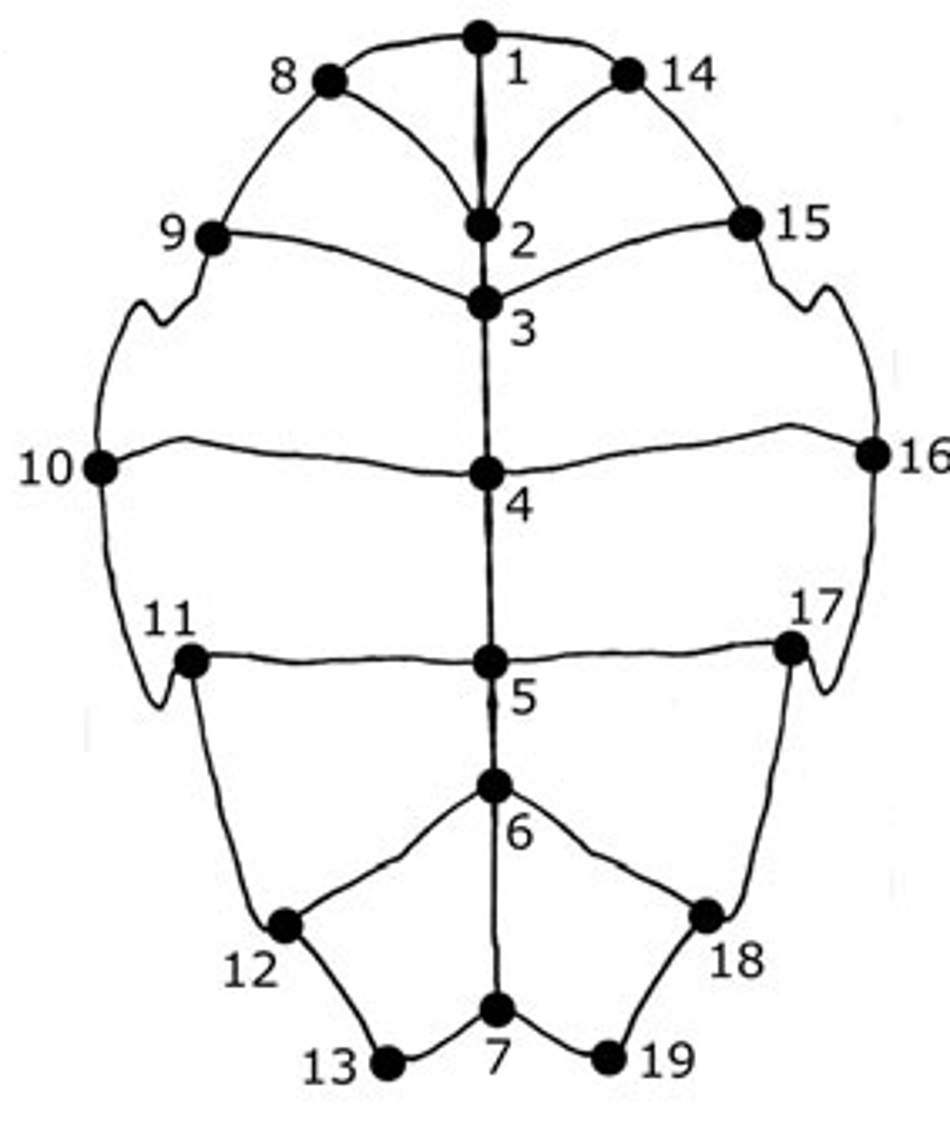
\includegraphics{figure/plastra}
  \caption{Depiction of general plastral shape of \textit{E. marmorata} and position of the 19 landmark used in this study. Anterior is towards the top of the figure.}
  \label{fig:plastra}
\end{figure}

\end{document}
